\documentclass{beamer}

\usepackage{amssymb,amsmath}
\usepackage{graphicx}
\usepackage{url}
\usepackage{color}
\usepackage{relsize}		% For \smaller
\usepackage{url}			% For \url
\usepackage{epstopdf}	% Included EPS files automatically converted to PDF to include with pdflatex
\usepackage{pagenote}[continuous,page]

%For MindMaps
% \usepackage{tikz}%
% \usetikzlibrary{mindmap,trees,arrows}%

%%% Color Definitions %%%%%%%%%%%%%%%%%%%%%%%%%%%%%%%%%%%%%%%%%%%%%%%%%%%%%%%%%
%\definecolor{bordercol}{RGB}{40,40,40}
%\definecolor{headercol1}{RGB}{186,215,230}
%\definecolor{headercol2}{RGB}{80,80,80}
%\definecolor{headerfontcol}{RGB}{0,0,0}
%\definecolor{boxcolor}{RGB}{186,215,230}

%%% Save space in lists. Use this after the opening of the list %%%%%%%%%%%%%%%%
%\newcommand{\compresslist}{
%	\setlength{\itemsep}{1pt}
%	\setlength{\parskip}{0pt}
%	\setlength{\parsep}{0pt}
%}

%\setbeameroption{show notes on top}

% You should run 'pdflatex' TWICE, because of TOC issues.

% Rename this file.  A common temptation for first-time slide makers
% is to name it something like ``my_talk.tex'' or
% ``john_doe_talk.tex'' or even ``discrete_math_seminar_talk.tex''.
% You really won't like any of these titles the second time you give a
% talk.  Try naming your tex file something more descriptive, like
% ``riemann_hypothesis_short_proof_talk.tex''.  Even better (in case
% you recycle 99% of a talk, but still want to change a little, and
% retain copies of each), how about
% ``riemann_hypothesis_short_proof_MIT-Colloquium.2000-01-01.tex''?

\mode<presentation>
{
  % A tip: pick a theme you like first, and THEN modify the color theme, and then add math content.
  % Warsaw is the theme selected by default in Beamer's installation sample files.

  %%%%%%%%%%%%%%%%%%%%%%%%%%%% THEME
  %\usetheme{Madrid}		% No subsection
  \usetheme{AnnArbor}  % Subsection on top, no color


  %\usetheme{Antibes}
  %\usetheme{Bergen}
  %\usetheme{Berkeley}		% bem bacana - menu esquerdo
  %\usetheme{Berlin}
  %\usetheme{Boadilla}
  %\usetheme{boxes}
  %\usetheme{CambridgeUS}		% bem bacana - menu superior
  %\usetheme{Copenhagen}
  %\usetheme{Darmstadt}
  %\usetheme{default}
  %\usetheme{Dresden}
  %\usetheme{Frankfurt}
  %\usetheme{Goettingen}
  %\usetheme{Hannover}		% bem bacana - menu esquerdo
  %\usetheme{Ilmenau}
  %\usetheme{JuanLesPins}
  %\usetheme{Luebeck}
  %\usetheme{Malmoe}
  %\usetheme{Marburg}		% bem bacana - menu direito
  %\usetheme{Montpellier}
  %\usetheme{PaloAlto}		% bem bacana - menu esquerdo
  %\usetheme{Pittsburgh}
  %\usetheme{Rochester}		%bacana
  %\usetheme{Singapore}
  %\usetheme{Szeged}
  %\usetheme{Warsaw}

  %%%%%%%%%%%%%%%%%%%%%%%%%%%% COLOR THEME
  %\usecolortheme{default}		% branco, azul clarinho
  \usecolortheme{crane}		% Very yellow (ok)

  %\usecolortheme{albatross}		% azul escuro, massa
  %\usecolortheme{beetle}		% cinza, menu azul
  %\usecolortheme{dolphin}		% azul e branco, legal
  %\usecolortheme{dove}			% cinza e branco, feio
  %\usecolortheme{fly}			% todo cinza, horrível
  %\usecolortheme{lily}			% parece o default
  %\usecolortheme{orchid}		% azul e branco, ok
  %\usecolortheme{rose}			% branco e violeta-claro, bonito
  %\usecolortheme{seagull}		% cinza, feio
  %\usecolortheme{seahorse}		% nhé, meio feio
  %\usecolortheme{sidebartab}		% Azul, branco, destaque na tab, interessante
  %\usecolortheme{structure}		% bichado
  %\usecolortheme{whale}		% Azul e branco, bem bonito

  %%%%%%%%%%%%%%%%%%%%%%%%%%%% OUTER THEME
  \useoutertheme{default}
  %\useoutertheme{infolines}
  %\useoutertheme{miniframes}
  %\useoutertheme{shadow}
  %\useoutertheme{sidebar}
  %\useoutertheme{smoothbars}
  %\useoutertheme{smoothtree}
  %\useoutertheme{split}
  %\useoutertheme{tree}

  %%%%%%%%%%%%%%%%%%%%%%%%%%%% INNER THEME
  \useinnertheme{circles}
  %\useinnertheme{default}
  %\useinnertheme{inmargin}
  %\useinnertheme{rectangles}
  %\useinnertheme{rounded}

  %%%%%%%%%%%%%%%%%%%%%%%%%%%%%%%%%%%

  \setbeamercovered{invisible} % or whatever (possibly just delete it)
  % To change behavior of \uncover from graying out to totally
  % invisible, can change \setbeamercovered to invisible instead of
  % transparent. apparently there are also 'dynamic' modes that make
  % the amount of graying depend on how long it'll take until the
  % thing is uncovered.

}


% Get rid of nav bar
\beamertemplatenavigationsymbolsempty

% Use short top
%\usepackage[headheight=12pt,footheight=12pt]{beamerthemeboxes}
%\addheadboxtemplate{\color{black}}{
%\hskip0.5cm
%\color{white}
%\insertshortauthor \ \ \ \
%\insertframenumber \ \ \ \ \ \ \
%\insertsection \ \ \ \ \ \ \ \ \ \ \ \ \ \ \ \ \  \insertsubsection
%\hskip0.5cm}
%\addheadboxtemplate{\color{black}}{
%\color{white}
%\ \ \ \
%\insertsection
%}
%\addheadboxtemplate{\color{black}}{
%\color{white}
%\ \ \ \
%\insertsubsection
%}

% Insert frame number at bottom of the page.
% \usefoottemplate{\hfil\tiny{\color{black!90}\insertframenumber}}

%% makes the ppagenote command for figure references at the end.

\usepackage[english]{babel}
%qq\usepackage[latin1]{inputenc}
\usepackage{CJKutf8}
\usepackage{subfigure}

\usepackage{times}
\usepackage[T1]{fontenc}

\makepagenote
\renewcommand{\notenumintext}[1]{}
\newcommand{\ppagenote}[1]{\pagenote[Page \insertframenumber]{#1}}

\title[Programming Challenges]{GB20602 - Programming Challenges}
\author[Claus Aranha]{Claus Aranha\\{\footnotesize caranha@cs.tsukuba.ac.jp}}
\institute[U. Tsukuba]{University of Tsukuba, Department of Computer Sciences}



\usepackage{tikz}
\usetikzlibrary{arrows,shapes}
\tikzstyle{vertex}=[circle,fill=black!25,minimum size=10pt,inner sep=0pt]
\tikzstyle{blue vertex}=[circle,fill=blue!100,minimum size=10pt,inner sep=0pt]
\tikzstyle{red vertex}=[circle,fill=red!100,minimum size=10pt,inner sep=0pt]
\tikzstyle{edge} = [draw,thick,-]
\tikzstyle{red edge} = [draw, line width=5pt,-,red!50]
\tikzstyle{black edge} = [draw, line width=5pt,-,black!20]
\tikzstyle{weight} = [font=\smaller]

\title[GB21802]{GB21802 - Programming Challenges}
\subtitle[]{Week 9 - Programming Challenges Remix!}
\author[Claus Aranha]{Claus Aranha\\{\footnotesize caranha@cs.tsukuba.ac.jp}}
\institute{College of Information Science}
\date{2015-06-23,26\\{\tiny Last updated \today}}

\begin{document}

\section{Introduction}
\subsection{Title}
\begin{frame}
\maketitle
\end{frame}

\subsection{Class Notes}

\subsection{Grade Discussion}

\begin{frame}
  \frametitle{Grade Dates}

  \begin{itemize}
  \item Final Submission Date: 7/6
    \bigskip

  \item Grade Announcement: 7/9 (on Manaba)
    \bigskip

  \item Grade Registration: 7/13
  \end{itemize}  
\end{frame}



%%%%%%%%%%%%%%%%%%%%%%%%%%%%%%%%%%%%%%%%
\section{Solving Problems}
\subsection{Solving Problems}
\begin{frame}
  \frametitle{Course Summary -- Solving a problem}

  {\smaller
    \begin{block}{}
      In this course, we studied and practice many ways
      to solve problems using computer algorithms. Many
      problems can be imagined as \emph{searches}.
    \end{block}

    \vfill
    
    General Problem Solving:
    \begin{itemize}
    \item Identify the \structure{full search approach}
    \item Think about edge and special cases
    \item See if a better algorithm \structure{is needed}
    \end{itemize}
    
  }
  
\end{frame}

\begin{frame}
  \frametitle{Course Summary -- Topics Approached}

  {\smaller
    \begin{exampleblock}{}
      In this course we also saw many examples of \structure{specific}
      algorithms for problems.
    \end{exampleblock}

    \vfill

    \begin{itemize}
    \item Graphs (Minimum spanning tree, Bellman-Ford APSP, $\ldots$)
    \item Mathematics (Eristhenes Sieve, Prime Factoring)
    \item Computational Geometry (Convex Hull)
    \item String (Knuth-Morris-Prat, suffix trie)
    \end{itemize}
    
  }
  % Course lessons and representative algorithms
\end{frame}

\begin{frame}
  \frametitle{Course Summary -- Multi-Problems}

  The most interesting problems are those that \structure{mix two or
    more} different algorithms. Or \structure{require variations} of
  standard algorithms.

  \bigskip

  This week, we will try to solve together some of these more
  interesting problems.
\end{frame}

\section{Interesting Problems}
\subsection{Problem Description}


\begin{frame}[fragile]
  \frametitle{UVA 10937 -- Blackbeard the Pirate}

  {\smaller

    \begin{block}{}
      Blackbeard has to \structure{collect all treasures} (up to 10)
      in the island. He \alert{cannot cross} water or trees, and he
      must stay 1 square away from natives.

      \medskip

      Black beard speed is 1 square / second. How long does it take
      to get all treasure and return to the ship?
    \end{block}
    
\begin{verbatim}
10 10
~~~~~~~~~~       ~ -- Water, can't cross
~~!!!###~~       # -- Trees, can't cross
~##...###~       ! -- Treasure, get these!
~#....*##~       . -- Just sand
~#!..**~~~       @ -- Landing point, return here.
~~....~~~~
~~~....~~~       The solution for this case is: 32
~~..~..@~~       How would YOU solve this problem?
~#!.~~~~~~
~~~~~~~~~~
0 0
\end{verbatim}
}
\end{frame}

\begin{frame}
  \frametitle{UVA 10937 -- Blackbeard the Pirate}

  How would you solve this problem?

  \vfill

  \begin{itemize}
  \item Which algorithm do you suggest?
    \bigskip
    
  \item What is the complexity of that algorithm?

    \bigskip
  \item Where do you need to be careful?
  \end{itemize}

  \bigskip

  \alert{Quiz} -- What is the complexity of the problem for full
  recursive search? (Map size $50x50$, number of treasures is $10$)
  
\end{frame}

\subsection{Problem Solution -- Decomposition}
\begin{frame}[fragile]
  \frametitle{UVA 10937 -- Blackbeard the Pirate}

  {\smaller

    \begin{block}{Breaking the problem into parts}
      One way to solve this problem is to break it into two parts:
      \begin{enumerate}
      \item Extract a weighted distance graph from the input map
      \item Solve the TSP for the graph
      \end{enumerate}
    \end{block}

\begin{verbatim}
10 10
~~~~~~~~~~       ~ -- Water, can't cross
~~!!!###~~       # -- Trees, can't cross
~##...###~       ! -- Treasure, get these!
~#....*##~       . -- Just sand
~#!..**~~~       @ -- Landing point, return here.
~~....~~~~
~~~....~~~       
~~..~..@~~       
~#!.~~~~~~
~~~~~~~~~~
0 0
\end{verbatim}
  }
\end{frame}

\begin{frame}[fragile]
  \frametitle{UVA 10937 -- Blackbeard -- Extracting the graph}

  {\smaller
\begin{verbatim}
10 10
~~~~~~~~~~  ##########  # -- Obstacle (waters and trees)
~~!!!###~~  ##345#####  X -- Obstacles (natives, just for clarity)
~##...###~  ###..X####  . -- Path
~#....*##~  ##..XXX###  0-9 -- Nodes
~#!..**~~~  ##2.XXX###  
~~....~~~~  ##..XX####
~~~....~~~  ###....###     
~~..~..@~~  ##..#..0##     
~#!.~~~~~~  ##1.######
~~~~~~~~~~  ##########
0 0
\end{verbatim}

\begin{itemize}
\item We can simply the graph into obstacles, paths and goals
\item We are only interested in the treasures and goals, so how to find the
  pairwise distance between treasures?
\item \alert{Answer}: \only<2>{BFS from each treasure/start point}
\item The result is a small graph with {\bf at most} 11 vertices.
\end{itemize}

  }
\end{frame}

\begin{frame}[fragile]
  \frametitle{UVA 10937 -- Blackbeard -- Extracting the graph}
  \begin{columns}
    \column{0.5\textwidth}
    
  {\smaller
\begin{verbatim}
##########  
##345#####  
###..X####  
##..XXX###     BFS from each vertex
##2.XXX###     ------------------->
##..XX####     Not all paths shown
###....###     
##..#..0##     
##1.######
##########
\end{verbatim}}

    \column{0.5\textwidth}
  \begin{center}
    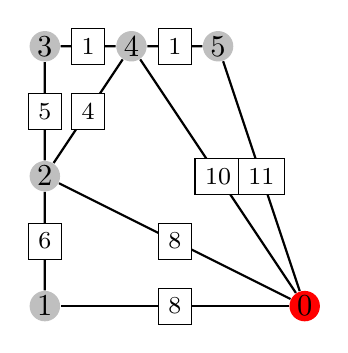
\begin{tikzpicture}[transform shape,label/.style={thin, draw=black, align=center,fill=white,font=\smaller},scale=1.1]
      \node[red vertex] (S) at (3,0) {0};
      \node[vertex] (ta) at (0,0) {1};
      \node[vertex] (tb) at (0,1.5) {2};
      \node[vertex] (tc) at (0,3) {3};
      \node[vertex] (td) at (1,3) {4};
      \node[vertex] (te) at (2,3) {5};
      \draw[edge] (S) -- node[label] {$8$} (ta);
      \draw[edge] (S) -- node[label] {$8$} (tb);
      \draw[edge] (S) -- node[label] {$10$} (td);
      \draw[edge] (td) -- node[label] {$1$} (tc);
      \draw[edge] (td) -- node[label] {$1$} (te);
      \draw[edge] (td) -- node[label] {$4$} (tb);
      \draw[edge] (tb) -- node[label] {$6$} (ta);
      \draw[edge] (S) -- node[label] {$11$} (te);
      \draw[edge] (tb) -- node[label] {$5$} (tc);
    \end{tikzpicture}
  \end{center}
  \end{columns}

  \begin{center}
    How do we find the minimal cycle starting in {\bf S}, passing by all vertices?
  \end{center}
\end{frame}

%% Explain TSP with DP and bit (Page 110)

\subsection{Traveling Salesman Problems}

\begin{frame}
  \frametitle{The Traveling Salesman Problem (TSP)}

  {\smaller
    \begin{block}{Problem Definition}
      You have $n$ cities, and their distances. Calculate the cost of
      the \structure{tour} that starts and ends at a city $s$, passing
      through all other cities.

      \medskip

      Exactly what we need! The path for all treasure!
  \end{block}
  \begin{center}
    \includegraphics[width=0.6\textwidth]{../img/tsp_example}
  \end{center}

  In the graph above, we have $n=4$ cities and the minimal tour is
  A-B-C-D-A, with cost $20+30+12+35=97$.

  \medskip

  \alert{QUIZ:} What is the cost of solving TSP with complete search?  
  }
  
  \hrulefill

  \hfill{\tiny Image from Steven Halim -- ``Competitive Programming''}
  
\end{frame}

\begin{frame}
  \frametitle{Characteristics of TSP}

  {\smaller
    \begin{block}{}
      \begin{itemize}        
      \item A complete search for TSP costs $O(n!*n)$ -- \alert{Search
        each city permutation}.
      \item TSP is a {\bf NP-hard} problem. This means that there is
        no known polinomial algorithm to solve it.
      \item \alert{However!} For small values of $n$, there are some
        hacks to make the solution faster.
      \end{itemize}
    \end{block}

    \begin{exampleblock}{DP approach to TSP}
      The complete search for the TSP contains many \alert{repeated subsolutions}:
      \begin{itemize}
      \item S--A--B--C--$\ldots$--S
      \item S--B--A--C--$\ldots$--S
      \end{itemize}
      The minimum cost for C--$\ldots$--S is the same. Can we use
      \emph{memoization} to remember this cost?
    \end{exampleblock}
  }
\end{frame}

\begin{frame}
  \frametitle{DP approach to TSP (1) -- Idea}

  {\smaller
    \begin{block}{}
      \begin{itemize}
      \item We have already visited the cities $S = \{s_1,s_2,\ldots,s_n\}, s_i \neq 0$
      \item We are {\bf now} in city $s_k \in S$
      \item What is the shortest path from $s_k$ to $0$, that passes in all cities $s_j \notin S$ ?
      \end{itemize}

      DP induction: shortest\_path($S$,$s_k$)
    \end{block}
    \begin{center}
      \includegraphics[width=0.7\textwidth]{img/DP_TSP}
    \end{center}
  }
\end{frame}

\begin{frame}
  \frametitle{DP approach to TSP (2) -- Recurrence}

  {\smaller
    \begin{center}
      \includegraphics[width=0.5\textwidth]{img/DP_TSP}
    \end{center}
    \begin{block}{DP Recurrence}
      \begin{itemize}
      \item We have visited all cities, and must return to the origin:\\
        shortest\_path($S_{\text{all}},s_k$) = $D(s_k,0)$
      \item We have visited some cites ($S$), and must find the next one:\\
        shortest\_path($S,s_k$) = {\bf minimum}$(D(s_k,s_i) + \text{shortest\_path}(S\cup s_i,s_i))$
      \item Initial call:\\
        shortest\_path($\emptyset$,0)
      \end{itemize}
    \end{block}
  }
\end{frame}

\begin{frame}
  \frametitle{DP approach to TSP (3) -- Implementation}

  {\smaller
    \begin{exampleblock}{}
      \begin{itemize}
      \item Our DP table is (\emph{all sets},\emph{all cities}) -- $2^n * n$
      \item We can represent a set of cities using a \structure{bitmask}
      \item At each call, we loop through all cities, so the complexity is $(O(2^n*n^2))$

        \bigskip

      \item TSP using full search: $O(n!*n)$
      \item TSP using DP: $O(2^n*n^2)$ -- Still low, but much better!        
      \end{itemize}
    \end{exampleblock}
  }
\end{frame}

\begin{frame}[fragile]
  \frametitle{DP approach to TSP (4) -- Sample Code}

{\smaller
  \begin{exampleblock}{}
\begin{verbatim}
int dp[n][1<<n] = -1
start = 0

visit(p,v):
   if (v == (1<<n) - 1):
      return cost[p][start]
   if dp[p][v] != -1
      return dp[p][v]

   tmp = MAXINT
   for i in n:
       if not(v && (1 << i):
           tmp = min(tmp,
                     cost[p][i] + visit(i, v | (1<<i)))

   dp[p][v] = tmp
   return tmp
\end{verbatim}
  \end{exampleblock}}
\end{frame}


\subsection{UVA 10003 -- Cutting Sticks}
\begin{frame}
  \frametitle{UVA 10003 -- Cutting Sticks}
  
  {\smaller
  \begin{block}{Problem Description}
    Given a stick of length $1 \leq l \leq 1000$ and $1 \leq n \leq
    50$ cuts (positions) to be made, the cost of a cut is given by the length of 
    the stick being cut.

    \medskip

    Find a cutting sequence that minimizes the cost of cutting the stick.
  \end{block}
  
  \medskip

  \structure{Example:} $l=100, n=3, cuts=\{25,50,75\}$

  \begin{center}
    \includegraphics[width=0.6\textwidth]{../img/cuttingsticks}
  \end{center}

  \begin{itemize}
  \item Sequence 1: 25, 50, 75. Cost: 100 + 75 + 50 = 225
  \item Sequence 2: 50, 25, 75. Cost: 100 + 50 + 50 = 200
  \end{itemize}

  \begin{block}{}
  What is the recurrence to find the minimum cost?
  \end{block}
  }
\end{frame}

\begin{frame}
  \frametitle{Cutting Sticks -- Recurrence}
  {\smaller
    \structure{Basic Idea}: Price(start,end) = end-start + Price(start,cut) + Price(cut,end)

    \medskip

    \alert{Problem}: Using start/end, we have 1000*1000 states.

    \medskip
    
    \structure{Solution}: We use cut indexes instead! (50*50 states)

    \vfill

    \begin{block}{Recurrence using cut index:}
    \begin{itemize}
    \item Price(i,i+1) = 0 
    \item Price(i,j) = min(Size[j] - Size[i] + Price(i,k) + Price(k,j))\\
      (for all $i < k < j$)        
    \end{itemize}
    \end{block}


    \medskip
    
    Note that the recurrence costs $O(n)$, and the table size is $O(n^2)$, 
    so the total cost is $O(n^3)$ }
\end{frame}


\section{More Examples}
\subsection{DP on Math Problems}

\begin{frame}
  \frametitle{DP on Math Problems}
  Many math problems can be implemented as DP:
  \begin{itemize}
  \item Combinatoric problems often have recursive formulas, and
    overlapping subproblems;
    \begin{itemize}
    \item Fibonacci Number: $f(n) = f(n-1)+f(n-2)$
    \end{itemize}
  \item Probability problems often require you to search the entire
    probability space (tree). These trees usually have overlapping branches.
  \item Maths problems on static data (sum, min, max)
  \end{itemize}
\end{frame}

% TODO: Add a DP math example (Yahtzee?)
%\begin{frame}
%  \frametitle{DP on Math Problems}
%\end{frame}


\begin{frame}
  \frametitle{DP on Strings}
  \begin{itemize}
  \item edit distance, substring manipulation, etc.
  \item Usually, we don't send the string in the recurrence, but
    \structure{indexes on the string}\\
    %% TODO: Add an string problem
  \end{itemize}
\end{frame}

\begin{frame}
  \frametitle{DP Issues}
  
  {\small
  \begin{itemize}
  \item Many DP problems look like ``non DP'' problems. 

    \begin{block}{Example}
      Select positions for a set of flags that cover a certain
      radius, in order to maximize area coverage. 

      \medskip
      
      The area calculation requires geometry, but the flag selection is 
      usually DP.
    \end{block}
    
    \medskip
    
  \item Some problem have sub-problems, but they are not overlapping.\\
    (In this case, DP will not work, but maybe Divide and Conquer?)
  \end{itemize}}
\end{frame}

\subsection{A few more problems}
% Add discussion for a few more problems


\section{Conclusion}
\subsection{Conclusion}
\begin{frame}
  \frametitle{That's all for DP!}
  This is what we've seen for weeks 3 and 4:

  \begin{itemize}
  \item DP = Complete Search + State table;
  \item Good when many \structure{overlapping subproblems} exist;
  \item Top-Down (recursive) and Bottom-Up (nested loops);
  \item Classical DP problems;
  \item (some!) non-classical DP problems;
  \end{itemize}

  \vfill

  For the next two weeks, the theme will be \structure{graph algorithms}!
\end{frame}

\subsection{Week 4 Problems}
\begin{frame}
  \frametitle{Problems for Week 4}
  \begin{itemize}
  \item Collecting Beepers
  \item Shopping Trip
  \item Bar Codes
  \item Cutting Sticks
  \item String Popping
  \item Divisibility
  \item Marks Distribution
  \item Squares
  \end{itemize}

\end{frame}

\begin{frame}
  \frametitle{World Finals Problem - 2016 Problem C}
  {\smaller
  \begin{block}{Problem Description -- Ceiling Function}
    Given $n$ arrays with $K$ values each, each array 
    is organized in a binary search tree in the order of input. 

    \bigskip
    
    In other words, the first element is the root, the second
    is the left child of the root if smaller, right child if bigger, 
    so on.

    \bigskip

    Count the number of different trees generated by the input data.    
  \end{block}

  \begin{center}
    \includegraphics[width=0.7\textwidth]{../img/worldfinal2016}
  \end{center}

  }
\end{frame}


\end{document}



